\title{Study Guide for Midterm 1 for Algebra-Based Physics: Electricity and Magnetism}
\author{Dr. Jordan Hanson - Whittier College Dept. of Physics and Astronomy}
\date{\today}
\documentclass[10pt]{article}
\usepackage[a4paper, total={18cm, 27cm}]{geometry}
\usepackage{outlines}
\usepackage[sfdefault]{FiraSans}
\usepackage{hyperref}
\usepackage{graphicx}
\begin{document}
\maketitle

\textbf{Instructions:} Work each problem before looking at the given answer.  See if you first understand the problem \textit{conceptually}, then work out the mathematics, then end with plugging in relevant data. \\ \vspace{0.25cm}

\textbf{Memory Bank:}
\begin{enumerate}
\item Coulomb Force: $\vec{F} = k \frac{q_1 q_2}{r^2}\hat{r}$
\item $k = 9 \times 10^{9}$ N C$^{-2}$ m$^{2}$
\item $q_e = 1.6 \times 10^{-19}$ C
\item Mass of a proton: $1.67 \times 10^{-27}$ kg
\item Electric field and charge: $\vec{F} = q \vec{E}$
\item Field of infinite wire of charge density $\lambda$: $\vec{E}(z) = \frac{2k\lambda}{z}\hat{z}$
\item Field of two oppositely charged infinite planes, with charge density $\sigma$: $\vec{E}(z) = \frac{\sigma}{\epsilon_0}\hat{z}$
\item $\epsilon_0 \approx 8.85 \times 10^{-12}$ F/m
\item Dipole moment: $\vec{p} = q \vec{d}$
\item Torque on dipole moment: $\vec{\tau} = \vec{p} \times \vec{E}$
\item Electric flux: $\Phi = \vec{E} \cdot \vec{A} = EA \cos\theta$
\item Gauss' law: $\Phi = Q_{enc}/\epsilon_0$
\item Potential energy and voltage: $U = q\Delta V$
\item Voltage of a point charge: $V(r) = k\frac{q}{r}$
\item Voltage and E-field: $\vec{E} = -\frac{\Delta V}{\Delta x}$
\item Capacitance: $Q = CV$
\item Parallel plate capacitor: $C = \frac{\epsilon_0 A}{d}$
\item Adding two capacitors in series: $C_{tot}^{-1} = C_1^{-1} + C_2^{-2}$
\item Adding two capacitors in parallel: $C_{tot} = C_1 + C_2$
\item Definition of current: $I(t) = \frac{\Delta Q}{\Delta t}$
\item Drift velocity: $v_d = \frac{I}{nAq}$
\item Ohm's law: $V = IR$
\item \textbf{Adding two resistors in series} $R_{tot} = R_1 + R_2$
\item \textbf{Adding two resistors in parallel} $R_{tot}^{-1} = R_1^{-1} + R_2^{-2}$
\end{enumerate}

\clearpage

\begin{enumerate}
\item \textbf{Chapter 18, Electrostatics}
\begin{enumerate}
\item Protons in an atomic nucleus are typically $10^{-15}$ m apart. What is the electric force of repulsion between nuclear protons? \\ \vspace{2cm}
\item A charge $q_1 = 20 \mu$C and a charge $q_2 = 10 \mu$C are 1.0 m apart.  What is the force on a positive test charge halfway between them, and in which direction is the force? \\ \vspace{2cm}
\item Suppose the ``deflector'' in Fig. \ref{fig:e1} is $d=12$ cm long.  If a proton (mass given in Memory Bank) has an initial speed of $v=1.5 \times 10^{7}$ m/s, and the field depicted is $4.0 \times 10^5$ N/C, by how much has it been deflected?  (What is $d$?). \\ \vspace{2cm}
\begin{figure}
\centering
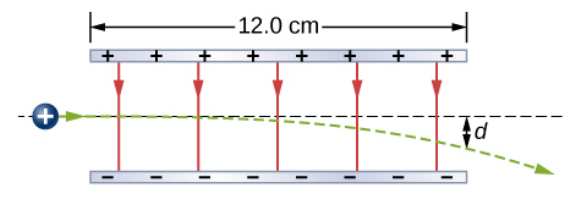
\includegraphics[width=0.45\textwidth]{figures/e1.png}
\caption{\label{fig:e1} A constant E-field deflecting a positive charge $q$.}
\end{figure}
\end{enumerate}
\item \textbf{Chapter 19, Voltage}
\begin{enumerate}
\item A lightning bolt strikes a tree, moving 20.0 C of charge through a potential difference of $10^8$ Volts. What energy was dissipated? \\ \vspace{2cm}
\item Consult again Fig. \ref{fig:e1}.  If the plates are 6 cm apart, and the field is still $4.0 \times 10^5$ N/C, what is the voltage difference between the plates? \\ \vspace{2cm}
\end{enumerate}
\item \textbf{Chapter 19, Capacitance}
\begin{enumerate}
\item Find the charge stored when 5.0 V is applied to an 8.00 pF capacitor. \\ \vspace{1cm}
\item Find the charge stored when 5.0 V is applied to two 8.00 pF capacitors \textit{in parallel}. \\ \vspace{1cm}
\item Find the charge stored when 5.0 V is applied to two 8.00 pF capacitors \textit{in series}. \\ \vspace{1cm}
\item Find the total capacitance in the circuit diagram of Fig. \ref{fig:c1}. \\ \vspace{2cm}
\begin{figure}
\centering
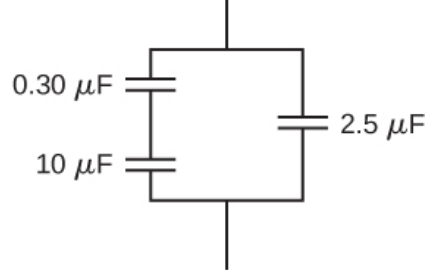
\includegraphics[width=0.4\textwidth]{figures/c1.png}
\caption{\label{fig:c1} Three capacitors connected together.}
\end{figure}
\end{enumerate}
\item \textbf{Chapter 20, Current and Ohm's law}
\begin{enumerate}
\item What current passes through a resistor with $R=1$ k$\Omega$, if the voltage applied is 12 V? \\ \vspace{1cm}
\item What current passes through two resistors with $R=1$ k$\Omega$, if the voltage applied is 12 V, and the resistors are connected \textit{in series}? Draw a circuit diagram. \\ \vspace{2cm}
\item What current passes through two resistors with $R=1$ k$\Omega$, if the voltage applied is 12 V, and the resistors are connected \textit{in parallel}? Draw a circuit diagram. \\ \vspace{2cm}
\end{enumerate}
\end{enumerate}
\end{document}